%%%%%%%%%%%%%%%%%%%%%%% file template.tex %%%%%%%%%%%%%%%%%%%%%%%%%
%
% This is a template file for RO 
%
% Copy it to a new file with a new name and use it as the basis
% for your article
%
%%%%%%%%%%%%%%%%%%%%%%%%   EDP Sciences  %%%%%%%%%%%%%%%%%%%%%%%%%%
%
\documentclass{ro}
\usepackage{amsmath, amsthm, amssymb, amsfonts, tikz, caption}
\usepackage{pgfplots}
\usetikzlibrary{matrix,chains,positioning,decorations,arrows}
%
%%%%%%%%%%%%%--PREAMBLE--%%%%%%%%%%%%%%%%%%
%%-----------------------------
%         ...........
%         your macros
%         ...........
%%-------------------------%%----
%%%%%%%%%%%%%%%--BODY--%%%%%%%%%%%%%%%%%%
\begin{document}
%%-----------------------------
%%      the top matter
%%-----------------------------
\title{Obtaining 3D Information from 2D Images Efficiently using Feature Extraction and Laser Dot Projection}
%
\author{Pratham Gandhi}
\author{Samuel Schuur}
%
\date{2018}
%

\begin{abstract} 
In this paper, the development and application of a novel system to computationally inexpensively determine a three dimensional model of a space from only a single image is presented, using applied machine learning and simple hardware components. Using feature classification of the relevant objects in the original scene, in collection with a physical grid of laser dots refracted across the scene, the system is able to quickly judge the nature of the object, its position in relation to other objects around it, and distance of those objects from the camera, functions where previously the accuracy of  commonly compromised on comparable approaches. The system is \begin{it}x\end{it} times more efficient on average than current industry leading approaches, and has potential applications in various fields requiring rapidly updating spatial awareness, including autonomous vehicles, defense, and architecture.
\end{abstract}

\maketitle

\pagebreak

\section{Introduction}


\section{Background}
\subsection{Neural Networks}
An Artificial Neural Network (ANN) is a computational model inspired by biological networks in the human brain which process large amounts of information.
\subsubsection{A Single Neuron}
The basic unit if a neural network is a neuron. A neuron is essentially a node in the graph which represents the neural network. Each neuron in an ANN, similar to a biological neuron, receives input from other neurons. Each input has an associated weight $W$, which is adjusted based on the importance of its corresponding input in the large picture of all the inputs to a neuron. Once it has acquired its inputs, a neuron will apply an activation function $f$, as shown below, to the weighted sum of its inputs to produce an output.
\input{Diagrams/Neuron.tex}

The function $f$ is a non-linear activation function. The role of the activation function is to create non-linearity in the output of a neuron, which is key because most real-world data in non linear and the purpose of neurons is to learn how to represent that data. Every activation function takes a single input and performs a mathematical operation on it in order to produce the final output. Common activation functions include:
\begin{itemize}
    \item Sigmoid: takes a value and squashes it to range 0-1. $\sigma(x) = \frac{1}{1+e^{-x}}$
    \item tahn: takes a value and squashes it to range [-1,1]. $\text{tahn}(x)=2\sigma(2x)-1$
    \item ReLU: stands for Rectified Linear Unit. Takes a value and replaces all negative values with 0. $f(x)=\text{max}(0,x)$
\end{itemize}

Constellation chooses to use sigmoid as the primary activation function due to its gradient nature, fixed range, and the fact that it is easier to differentiate values closer to one asympote or the other.
$$\text{input to activation}= (\sum\limits_{i=1}^n (x_i\times w_i))+b$$
$$\text{activation }f(x) = \frac{1}{1+e^{-x}}$$
$$\text{output}=\frac{1}{1+e^{-((\sum\limits_{i=1}^n (x_i\times w_i))+b))}}$$
\subsubsection{Feedforward Networks}
The feedforward neural network is the simplest and most widely applied type of ANN devised. Feedforward nets contain several neurons sorted into layers. Nodes from adjacent layers have connections, represented as edges on the graph, between them. Every connection, as discussed earlier, has a weight associated with it. \\

\begin{figure}[h]
\centering


\tikzset{every picture/.style={line width=0.75pt}} %set default line width to 0.75pt        

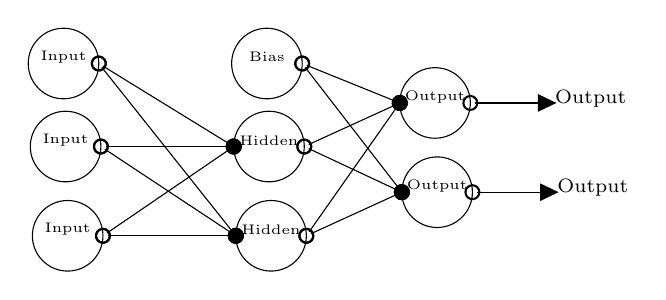
\begin{tikzpicture}[x=0.75pt,y=0.75pt,yscale=-1,xscale=1]
%uncomment if require: \path (0,300); %set diagram left start at 0, and has height of 300

\draw    (111, 77) circle [x radius= 17, y radius= 17]  ;
\draw    (130,78.23) -- (193,117) ;
\draw [shift={(193,117)}, rotate = 31.61] [color={rgb, 255:red, 0; green, 0; blue, 0 }  ][fill={rgb, 255:red, 0; green, 0; blue, 0 }  ][line width=0.75]      (0, 0) circle [x radius= 3.35, y radius= 3.35]   ;
\draw [shift={(128,77)}, rotate = 31.61] [color={rgb, 255:red, 0; green, 0; blue, 0 }  ][line width=0.75]      (0, 0) circle [x radius= 3.35, y radius= 3.35]   ;
\draw    (131.35,117) -- (193,117) ;
\draw [shift={(193,117)}, rotate = 0] [color={rgb, 255:red, 0; green, 0; blue, 0 }  ][fill={rgb, 255:red, 0; green, 0; blue, 0 }  ][line width=0.75]      (0, 0) circle [x radius= 3.35, y radius= 3.35]   ;
\draw [shift={(129,117)}, rotate = 0] [color={rgb, 255:red, 0; green, 0; blue, 0 }  ][line width=0.75]      (0, 0) circle [x radius= 3.35, y radius= 3.35]   ;
\draw    (131.94,158.68) -- (193,117) ;
\draw [shift={(193,117)}, rotate = 325.68] [color={rgb, 255:red, 0; green, 0; blue, 0 }  ][fill={rgb, 255:red, 0; green, 0; blue, 0 }  ][line width=0.75]      (0, 0) circle [x radius= 3.35, y radius= 3.35]   ;
\draw [shift={(130,160)}, rotate = 325.68] [color={rgb, 255:red, 0; green, 0; blue, 0 }  ][line width=0.75]      (0, 0) circle [x radius= 3.35, y radius= 3.35]   ;
\draw    (129.46,78.84) -- (194,160) ;
\draw [shift={(194,160)}, rotate = 51.51] [color={rgb, 255:red, 0; green, 0; blue, 0 }  ][fill={rgb, 255:red, 0; green, 0; blue, 0 }  ][line width=0.75]      (0, 0) circle [x radius= 3.35, y radius= 3.35]   ;
\draw [shift={(128,77)}, rotate = 51.51] [color={rgb, 255:red, 0; green, 0; blue, 0 }  ][line width=0.75]      (0, 0) circle [x radius= 3.35, y radius= 3.35]   ;
\draw    (130.96,118.3) -- (194,160) ;
\draw [shift={(194,160)}, rotate = 33.49] [color={rgb, 255:red, 0; green, 0; blue, 0 }  ][fill={rgb, 255:red, 0; green, 0; blue, 0 }  ][line width=0.75]      (0, 0) circle [x radius= 3.35, y radius= 3.35]   ;
\draw [shift={(129,117)}, rotate = 33.49] [color={rgb, 255:red, 0; green, 0; blue, 0 }  ][line width=0.75]      (0, 0) circle [x radius= 3.35, y radius= 3.35]   ;
\draw    (132.35,160) -- (194,160) ;
\draw [shift={(194,160)}, rotate = 0] [color={rgb, 255:red, 0; green, 0; blue, 0 }  ][fill={rgb, 255:red, 0; green, 0; blue, 0 }  ][line width=0.75]      (0, 0) circle [x radius= 3.35, y radius= 3.35]   ;
\draw [shift={(130,160)}, rotate = 0] [color={rgb, 255:red, 0; green, 0; blue, 0 }  ][line width=0.75]      (0, 0) circle [x radius= 3.35, y radius= 3.35]   ;
\draw    (112, 117) circle [x radius= 17, y radius= 17]  ;
\draw    (113, 160) circle [x radius= 17, y radius= 17]  ;
\draw    (209, 77) circle [x radius= 17, y radius= 17]  ;
\draw    (210, 117) circle [x radius= 17, y radius= 17]  ;
\draw    (211, 160) circle [x radius= 17, y radius= 17]  ;
\draw    (290, 96) circle [x radius= 17, y radius= 17]  ;
\draw    (291, 139) circle [x radius= 17, y radius= 17]  ;
\draw    (229.14,116.02) -- (273,96) ;
\draw [shift={(273,96)}, rotate = 335.46] [color={rgb, 255:red, 0; green, 0; blue, 0 }  ][fill={rgb, 255:red, 0; green, 0; blue, 0 }  ][line width=0.75]      (0, 0) circle [x radius= 3.35, y radius= 3.35]   ;
\draw [shift={(227,117)}, rotate = 335.46] [color={rgb, 255:red, 0; green, 0; blue, 0 }  ][line width=0.75]      (0, 0) circle [x radius= 3.35, y radius= 3.35]   ;
\draw    (229.13,118) -- (274,139) ;
\draw [shift={(274,139)}, rotate = 25.08] [color={rgb, 255:red, 0; green, 0; blue, 0 }  ][fill={rgb, 255:red, 0; green, 0; blue, 0 }  ][line width=0.75]      (0, 0) circle [x radius= 3.35, y radius= 3.35]   ;
\draw [shift={(227,117)}, rotate = 25.08] [color={rgb, 255:red, 0; green, 0; blue, 0 }  ][line width=0.75]      (0, 0) circle [x radius= 3.35, y radius= 3.35]   ;
\draw    (229.35,158.08) -- (273,96) ;
\draw [shift={(273,96)}, rotate = 305.11] [color={rgb, 255:red, 0; green, 0; blue, 0 }  ][fill={rgb, 255:red, 0; green, 0; blue, 0 }  ][line width=0.75]      (0, 0) circle [x radius= 3.35, y radius= 3.35]   ;
\draw [shift={(228,160)}, rotate = 305.11] [color={rgb, 255:red, 0; green, 0; blue, 0 }  ][line width=0.75]      (0, 0) circle [x radius= 3.35, y radius= 3.35]   ;
\draw    (230.14,159.02) -- (274,139) ;
\draw [shift={(274,139)}, rotate = 335.46] [color={rgb, 255:red, 0; green, 0; blue, 0 }  ][fill={rgb, 255:red, 0; green, 0; blue, 0 }  ][line width=0.75]      (0, 0) circle [x radius= 3.35, y radius= 3.35]   ;
\draw [shift={(228,160)}, rotate = 335.46] [color={rgb, 255:red, 0; green, 0; blue, 0 }  ][line width=0.75]      (0, 0) circle [x radius= 3.35, y radius= 3.35]   ;
\draw    (228.18,77.88) -- (273,96) ;
\draw [shift={(273,96)}, rotate = 22.01] [color={rgb, 255:red, 0; green, 0; blue, 0 }  ][fill={rgb, 255:red, 0; green, 0; blue, 0 }  ][line width=0.75]      (0, 0) circle [x radius= 3.35, y radius= 3.35]   ;
\draw [shift={(226,77)}, rotate = 22.01] [color={rgb, 255:red, 0; green, 0; blue, 0 }  ][line width=0.75]      (0, 0) circle [x radius= 3.35, y radius= 3.35]   ;
\draw    (227.44,78.86) -- (274,139) ;
\draw [shift={(274,139)}, rotate = 52.25] [color={rgb, 255:red, 0; green, 0; blue, 0 }  ][fill={rgb, 255:red, 0; green, 0; blue, 0 }  ][line width=0.75]      (0, 0) circle [x radius= 3.35, y radius= 3.35]   ;
\draw [shift={(226,77)}, rotate = 52.25] [color={rgb, 255:red, 0; green, 0; blue, 0 }  ][line width=0.75]      (0, 0) circle [x radius= 3.35, y radius= 3.35]   ;
\draw    (309.35,96) -- (346.5,96) ;
\draw [shift={(348.5,96)}, rotate = 180] [fill={rgb, 255:red, 0; green, 0; blue, 0 }  ][line width=0.75]  [draw opacity=0] (8.93,-4.29) -- (0,0) -- (8.93,4.29) -- cycle    ;
\draw [shift={(307,96)}, rotate = 0] [color={rgb, 255:red, 0; green, 0; blue, 0 }  ][line width=0.75]      (0, 0) circle [x radius= 3.35, y radius= 3.35]   ;
\draw    (310.35,139) -- (347.5,139) ;
\draw [shift={(349.5,139)}, rotate = 180] [fill={rgb, 255:red, 0; green, 0; blue, 0 }  ][line width=0.75]  [draw opacity=0] (8.93,-4.29) -- (0,0) -- (8.93,4.29) -- cycle    ;
\draw [shift={(308,139)}, rotate = 0] [color={rgb, 255:red, 0; green, 0; blue, 0 }  ][line width=0.75]      (0, 0) circle [x radius= 3.35, y radius= 3.35]   ;

\draw (111,74) node  [align=left] {{\tiny Input}};
\draw (112,114) node  [align=left] {{\tiny Input}};
\draw (113,157) node  [align=left] {{\tiny Input}};
\draw (209,74) node  [align=left] {{\tiny Bias}};
\draw (210,114) node  [align=left] {{\tiny Hidden}};
\draw (211,157) node  [align=left] {{\tiny Hidden}};
\draw (290,93) node  [align=left] {{\tiny Output}};
\draw (291,136) node  [align=left] {{\tiny Output}};
\draw (365,94) node  [align=left] {{\scriptsize Output}};
\draw (366,137) node  [align=left] {{\scriptsize Output}};


\end{tikzpicture}
\caption{An example of a feedforward neural network}
\subcaption{Note than an empty circle on an edge denotes a source and a filled circle on an edge denotes a sink.}
\end{figure}

A feedforward network can consist of three types of nodes:
\begin{enumerate}
    \item Input Nodes - Provide information from the outside world to the network, the set of which is called the "Input Layer". None of these nodes perform any computation.
    \item Hidden Nodes - Have no direct connection with outside world and only perform computations and transfer information from the input nodes to the output nodes. A set of these nodes in called a "Hidden Layer". Feedforward nets can have any number of hidden layers.
    \item Output Nodes - Collectively called the "Output Layer", these nodes perform computations and also transfer information from the network to the outside world
\end{enumerate}

In a feedforward network, information only moves forward, through the input nodes, hidden nodes, and then finally on to output nodes. There is no cycling or looping back through the network. Below is an abridged psuedocode version of the feedforward algorithm implemented in Constellation:
\def\BState{\State\hskip-\ALG@thistlm}
\begin{algorithm}
\caption{Modified Feed-Forward Algorithm}\label{euclid}
\begin{algorithmic}[1]
\Procedure{FeedForward:}{}
\State $\text{create and empty list of all layers' output}$ %
\State \emph{loop} \text{for each layer in network}: %
\State \enspace\enspace$\text{create empty list of this layer's outputs}$
\State \enspace\enspace$\text{biased input}\gets\sum\limits_{i=1}^n (x_i\times w_i)+b$
\State \enspace\enspace$\emph{loop} \text{ for each neuron in layer}:$
\State \enspace\enspace$\enspace\enspace \text{neuron output}\gets\sigma\text{(biased input)}$
\State \enspace\enspace$\enspace\enspace \text{layer's outputs}\gets\text{layer's outputs}+\text{neuron output}$
\State \enspace\enspace$\text{all outputs}\gets\text{all outputs}+\text{layer's output}$
\State $\Return \text{ all outputs}$ %
\EndProcedure
\end{algorithmic}
\end{algorithm}

\subsubsection{Training Using Back-Propagation}
It is possible to train a Multi-Layer Perceptron (MLP) Neural Network, a network which has at least one hidden layer, using a technique called back-propagation. Back-Propagation is a type of training approach which is called supervised learning, which means that the network is learning from labeled training data, where there is data is fed in, accompanied by classifications for each set of data which the network is told are correct. Each connection between nodes has a weight, which, as mentioned earlier, dictates the relevance of a specific input in the greater scope of all the inputs to a given neuron. The goal of learning is to assign correct weights to these edges in order to provide the most accurate classifications.

All weights are randomly assigned to begin with. Then, one by one, every training set is passed through the neural network, and, depending on how vast the difference desired and actual ouput of each layer, the error is propagated back to the previous layer. The error is noted and each weight is adjusted accordingly. This process is repeated using the provided data set until the network is outputting acceptably close classifications to the labeled classifications. Once this level is reached, the network can be passed previously unseen data and can use its trained weights to produce a classification. 

Below is an abridged psuedocode version of the backpropagation algorithm implemented in Constellation:
\def\BState{\State\hskip-\ALG@thistlm}
\begin{algorithm}
\caption{Modified Backpropagation Algorithm}\label{euclid}
\begin{algorithmic}[1]
\Procedure{backpropagate(network, input vector, targets):}{}
\State $\text{hidden outputs, outputs}\gets\text{feed\_forward(network, input vector)}$
\State $\emph{loop}\text{ for each output:}$
\State $\enspace\enspace\text{delta output}\gets\dot \sigma(\text{output})*(\text{output}-\text{target})$
\State $\emph{loop}\text{ for each output:}$
\State $\enspace\enspace\text{adjust weights of the }i\text{th neuron}$
\State $\text{// (hOutput = hidden output)}$
\State $\emph{loop}\text{ for each hidden output:}$
\State $\enspace\enspace\text{hidden delta}\gets\dot \sigma(\text{hOutput})*(\text{hOutput}-\text{next adjusted input})$
\State $\emph{loop}\text{ for each hidden output:}$
\State $\enspace\enspace\text{adjust weights of the }i\text{th hidden neuron}$
\EndProcedure
\end{algorithmic}
\end{algorithm}



%%-----------------------------
%%      your bibliography
%%-----------------------------
\end{document}

